% -*- latex -*-
%%%%%%%%%%%%%%%%%%%%%%%%%%%%%%%%%%%%%%%%%%%%%%%%%%%%%%%%%%%%%%%%
%%%%%%%%%%%%%%%%%%%%%%%%%%%%%%%%%%%%%%%%%%%%%%%%%%%%%%%%%%%%%%%%
%%%%
%%%% This text file is part of the theory writeup on the
%%%% Integrative Model for Parallelism,
%%%% copyright Victor Eijkhout (eijkhout@tacc.utexas.edu) 2014-8
%%%%
%%%% avoid.tex : master file for report IMP-06
%%%%
%%%%%%%%%%%%%%%%%%%%%%%%%%%%%%%%%%%%%%%%%%%%%%%%%%%%%%%%%%%%%%%%
%%%%%%%%%%%%%%%%%%%%%%%%%%%%%%%%%%%%%%%%%%%%%%%%%%%%%%%%%%%%%%%%
\documentclass[11pt,fleqn,preprint]{impreport}

\taccreportnumber{IMP-06}

\usepackage{geometry,fancyhdr,multirow,wrapfig}

\input setup

\title[communication avoiding]{Definition of a `communication avoiding' compiler in the Integrative Model\construction}
\author[Eijkhout]{Victor Eijkhout\thanks{{\tt
      eijkhout@tacc.utexas.edu}, Texas Advanced Computing Center, The
    University of Texas at Austin}}

\begin{document}
\maketitle

\begin{abstract}
IMP distributions are defined with respect to abstract processing entities,
leading to a concept of tasks, rather than processes. In a past note
we defined processors, and describe their interaction
as it arises from the task dataflow. In this note we extend that story, 
showing that certain arrangements of the task graph over processors
leads to a communication minimizing and latency hiding behaviour.
\end{abstract}

\section{Motivation}

On clusters the cost of communication can be high relatively to
the cost of computation. Hence, the \indexterm{overlapping computation
  and communication} (also known as \indexterm{latency hiding}) has
long been a goal of parallel programming.
%
On shared memory processors
with explicitly managed \indexterm{scratchpad} memory there is an
equivalent phenomenon: if data can be pushed to the scratchpad well in
advance of it being needed, we now hide the memory, rather than
network, latency.

Various techniques for latency hiding have been used. For instance,
the PETSc library~\cite{GrSm:petsc} splits the matrix-vector product
in local and non-local parts, so that the former can overlap the
communication of the latter.
%
Related, redundant computation in order to avoid communication is an
old idea~\cite{OpJo:improved-ssor}.

There is considerable work in the context of iterative methods for
linear system to mitigate the influence of communication.
\begin{itemize}
\item Reformulation of CG-like methods to reduce the number of inner
  products~\cite{ChGe:sstep,DAzEijRo:ppscicomp,Sa:practicalKrylov,Me:multicg}.
\item Multi-step methods that combine inner products, and can have
  better locality properties~\cite{ChGe:sstep}.
\item
  Overlapping either the preconditioner
  application or the matrix-vector product with a
  collective\cite{dehevo92:acta}. We will give a new variant, based
  on~\cite{Gropp:libraries}, that overlaps both.
\end{itemize}
Recently, the notion of redundant computation we revisited by Demmel
\emph{et al.}~\cite{Demmel2008IEEE:avoiding}, in so-called
`communication avoiding' methods. We will show how such methods
naturally arise in the IMP framework. This will be the main result of
this note.

\pagebreak

\section{Algorithmic latency hiding}
\input hiding

\section{Communication avoiding}

We explain the basic idea of the `communication avoiding' scheme. This
was originally proposed for iterative methods, such as $s$-step CG; in
the next section we will show that the IMP framework can realize this
in general.

\input gridupdate

\section{A `communication avoiding' framework}

We now show how the above scheme, proposed for iterative methods, can
be applied to general task graphs. This means that we can have a
`communication avoiding compiler', that turns an arbitrary computation
into a communication avoiding one.

\input avoiding

%% \section{Strategies for dealing with inter-process communication}
%% \input avoidstrategies

\vfill\pagebreak
\section{Simple examples}

\includegraphics{avoid-o3-b2}

\begin{multicols}{2}
\begin{verbatim}
Graph on node 0, execution of 1 macro steps:
k1 local execution: 0
  parallel time: 0
k3 receive: 2
k2 local execution: 5
  parallel time: 2
k3 local execution: 4
  parallel time: 2
total parallel time : 1*(0+2+2) = 4
overlap analysis:
  2 tasks to recv, 2 k2 parallel time
\end{verbatim}
\vfill\columnbreak
\begin{verbatim}
Graph on node 1, execution of 1 macro steps:
k1 local execution: 0
  parallel time: 0
k3 receive: 2
k2 local execution: 5
  parallel time: 2
k3 local execution: 4
  parallel time: 2
total parallel time : 1*(0+2+2) = 4
overlap analysis:
  2 tasks to recv, 2 k2 parallel time
\end{verbatim}
\end{multicols}

\vfill\pagebreak
\includegraphics{avoid-o4-b3}

\begin{multicols}{2}
\begin{verbatim}
Graph on node 0, execution of 1 macro steps:
k1 local execution: 1
   parallel time: 1
k3 receive: 3
k2 local execution: 8
   parallel time: 3
k3 local execution: 8
   parallel time: 4
 total parallel time : 1*(1+3+4) = 8
 overlap analysis:
   3 tasks to recv, 3 k2 parallel time
\end{verbatim}
\vfill\columnbreak
\begin{verbatim}
Graph on node 1, execution of 1 macro steps:
k1 local execution: 1
   parallel time: 1
k3 receive: 3
k2 local execution: 8
   parallel time: 3
k3 local execution: 8
   parallel time: 4
 total parallel time : 1*(1+3+4) = 8
 overlap analysis:
   3 tasks to recv, 3 k2 parallel time
\end{verbatim}

\end{multicols}

\section{Example: split computation of matrix-vector product}
\input avoidmvp

\section{DRAM semantics}
\input dram-semantics
\subsection{Prefetch streams}
\input prefetch

\section{Simulation}

\begin{figure}[p]
  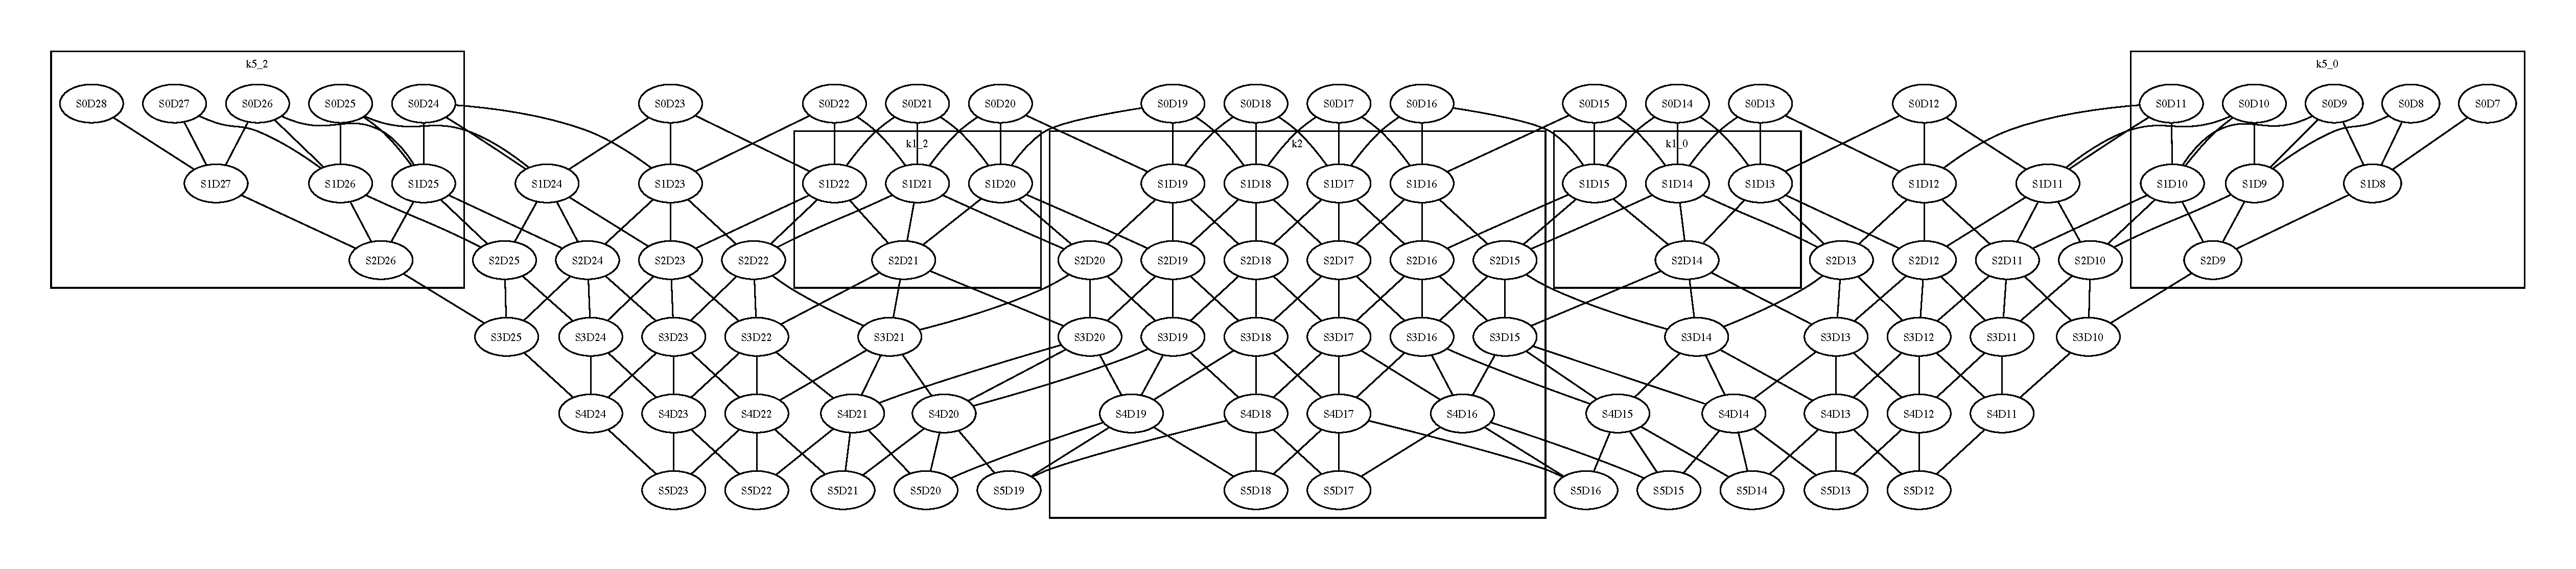
\includegraphics[scale=.17,angle=90]{nodegraph-1}
  \caption{Depiction of $k_1,k_2,k_3$ sets for a processor doing a 1D
    heat equation.}
  \label{fig:1dk123}
\end{figure}

We have written a simple simulator\footnote{The code can be found in
  the code repository~\cite{IMPcode-repo} under {\tt pocs/avoid}.} that takes a task graph and
identifies the $k_1,k_2,k_3$ sets. In figure~\ref{fig:1dk123} we
illustrate these sets for a one-dimensional case, but we note that the
analysis works on arbitrary task graphs.

We then simulate parallel runtimes by evaluating runtimes for the
following scenario:
\begin{itemize}
\item We use a strong scaling scenario where we have a given problem
  size and partitioning into tasks, as well the number of MPI nodes;
\item We set the ratio of message latency to floating point operation
  as fixed;
\item We evaluate the runtime as a function of the number of threads
  available for the task graph on an MPI node.
\end{itemize}
The prediction is that, with non-negligible latency, blocking will
reduce the running time more than the extra computation time from the
extended halo. Also, this effect will be more pronounced as the core
count increases, since this reduces the no-node computation time.

\begin{figure}[ht]
  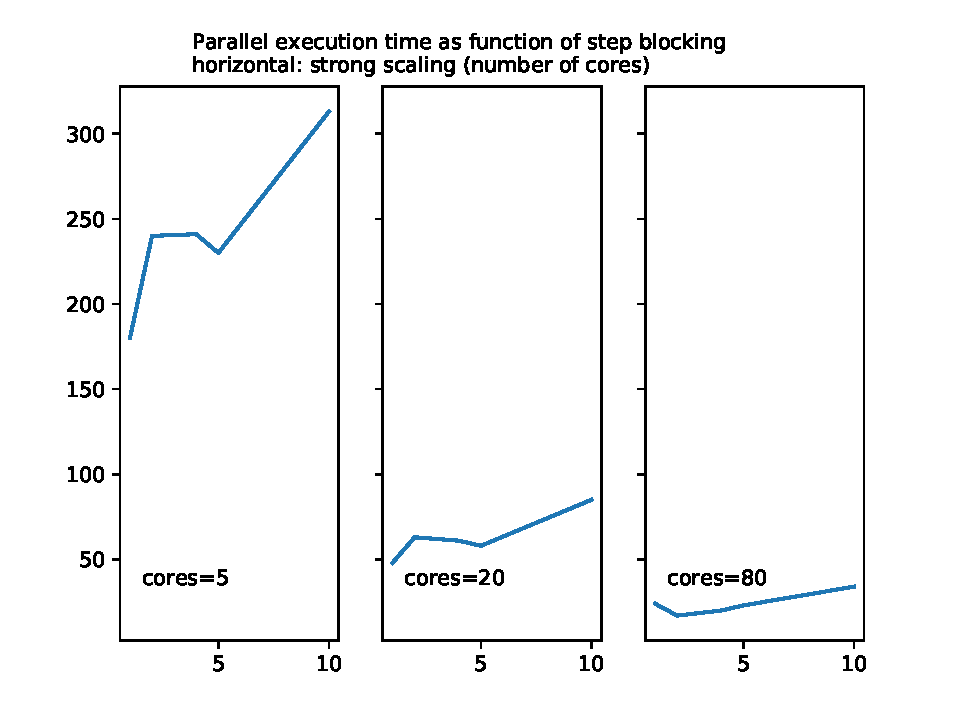
\includegraphics[scale=.4]{strongscale-1000}
  \caption{Runtime as a function of core count for moderate latency}
  \label{fig:lat1000}
\end{figure}
\begin{figure}[ht]
  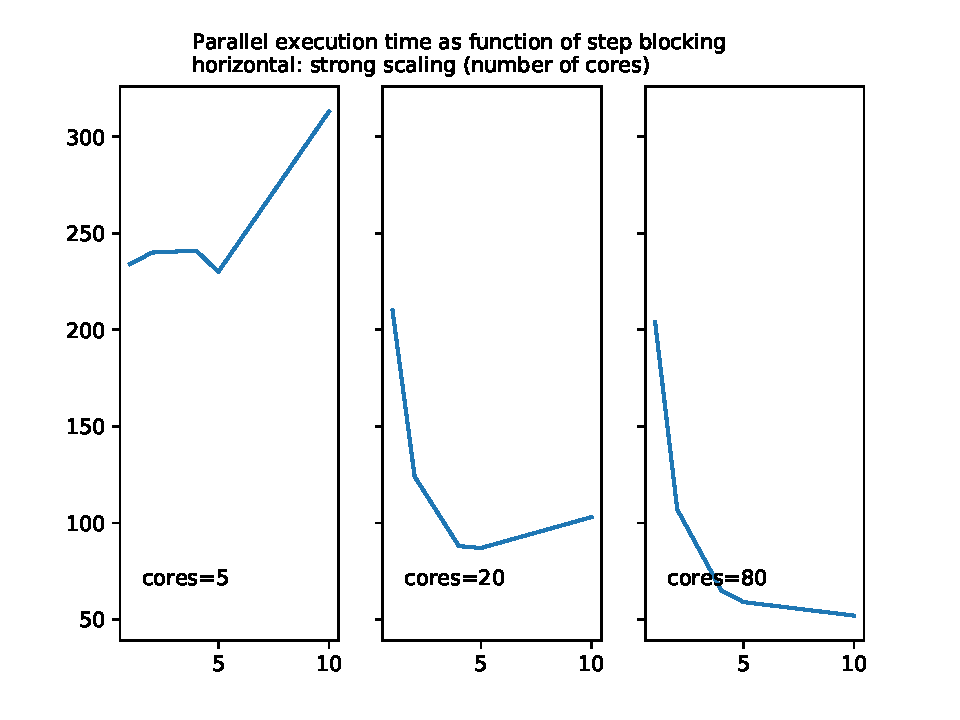
\includegraphics[scale=.4]{strongscale-10000}
  \caption{Runtime as a function of core count for high latency}
  \label{fig:lat10000}
\end{figure}
First, in figure~\ref{fig:lat1000} we use a low latency; we see that
only for very high thread count is there any gain. In
figure~\ref{fig:lat10000} we use a higher latency, and we see that
even for moderate thread counts blocking effects latency hiding.


\section{Conclusion}

We have discussed the concepts and prior work in latency hiding and
communication avoiding. We have shown that the IMP framework can turn
an arbitrary computation graph into a communication avoiding one by
judicious partitioning of the task graph, and duplicating certain tasks.

\bibliography{vle,imp}
\bibliographystyle{plain}

\end{document}
